% Chapter 5
\chapter{A Quasi-SERDES link Module} 
\label{chapter5}
%--------------------------------------------------------------------------
\section {Introduction}
As discussed in previous chapter high speed serial communication protocol Aurora 8B10B is an easy to use interface for communication between multiple Xilinx Virtex V FPGAs. But for the idea of this thesis work we plan to develop a interfacing link that is a generic module that can be used with CONNECT generated NoC and that uses GPIO pins available in any FPGA. This Quasi-SERDES interface module implements a quasi serialization of input data presented and also receives quasi serialized data from counterpart which is constructed back as output data. The module in its current state is designed for 24 bit data serialization / de-serialization (can be modified for any bit data) specifically designed for partitioned connect generated NoC with a flit width of 18 bits. This module is designed to operate at different clock rates to implement GALS architecture based application. With a few modifications this module can be made for any bit input data to 8 bit data stream and 8 bit data stream to reconstructed useful data. The Quasi-SERDES link interface module maintains an input buffer to ensure the lossless data transmission. Currently the buffer size is kept as 30 but an optimized design can reduce the buffer sizes.\\

\section{Features}
These are a few features that makes this module usable with NoC application and also for interfacing partitioned networks.
\begin{itemize} 
	\item{Clock synchronization and reset synchronization is handled in the module}
	\item{Any bit to 8-bit serialization/de-serialization}
	\item{Data reconstruction with validity check}
	\item{Flow control to ensure lossless data exchange}
	\item{Simple GPIO to GPIO interface}
	\item{Full duplex communication}
	\item{2 $\times$ 2 $\times$ n bit (input/output data)/8 number of clock cycles for data transfer. Therefore for 24 bit input data in 12 clock cycles 2bits/clock}
	\item{Buffer-full indication to routers so as to stop it from sending more data flits}
\end{itemize}

\begin{centering}
\begin{figure}[H]
  \centering
   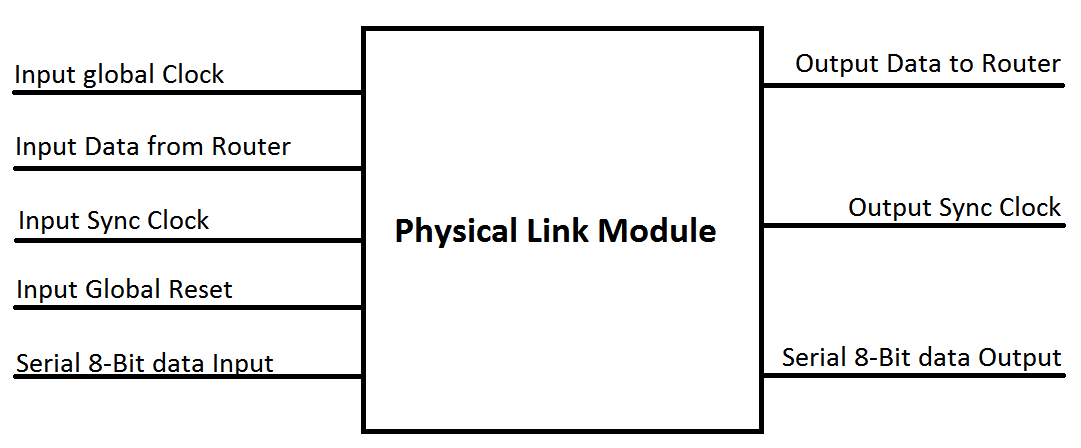
\includegraphics[scale=0.4]{./figs/physicalModule}
  \caption{\textbf{Quasi-SERDES Link Module}}
  \label{Quasi-SERDESModule}
\end{figure}
\end{centering}


\begin{table} [!h]
\caption{Quasi-SERDES Module Port Pins}
  \begin{center}
 \begin{tabular}{||c | c||} 
 \hline
    \textbf{PIN} & \textbf{DESCRIPTION} \\ \hline
    CLK & Input Clock \\
    rst\_n & Global Reset Input(Active low Reset)\\
    input\_data\_from\_router[17:0] & 18 bit input data (can be modified if needed)\\
    serial\_data\_in[7:0] & 8 bit data input (MSB first)\\
    serial\_data\_out[7:0] & 8 bit data output (MSB first)\\
    output\_data\_to\_router[17:0] & Reconstructed data received from 8 bit input \\
    sync\_clk\_in & input synchronization clock \\
    sync\_clk\_out & output synchronization clock \\
 \hline
\end{tabular}
\end{center}
\label{Quasi-SERDES_pins}
\end{table}

\section{Working Description}

This Quasi-SERDES module implements a simple protocol, whenever a valid data in presented as input from router keep it in buffer and start sending 8 bits at a time with MSB first. Similarly whenever a valid 8 bit MSB is received reconstruct output data and put the data on the output port to the router. The Quasi-SERDES link module recognizes a valid flit from router by checking its valid bit. Rest of the bits is treated as data and no processing or alteration is done to it.
\newpage
Key block in Verilog HDL: \\
The input data buffer filled when a valid data in received.
\begin{lstlisting}
if (input_data_from_router [17])
begin
	input_buffer_stack[a] <= input_data_from_router;
	en_recv_to_router_port <= 1;
	a = a +1;
	input_buffer_ready <= 1;
end
\end{lstlisting}

Sending the input data stored in buffer 8 bits at a time.\\*
\begin{lstlisting}
Case (e)
	1:
	begin	
		serial_data_out <= {6'b0, output_buffer [17:16]}; // Zero Padding
		e <= 2;
	end
	2:
	begin	
		serial_data_out <= output_buffer [15:8];
		e <= 3;
	end
	3:
	begin
		serial_data_out <= output_buffer [7:0];
		e = 0;
	end
\end{lstlisting}

Similarly two more blocks for receiving 8 bits data and sending  bits output data to router.



\section{Performance Parameters}
\begin{enumerate} 
	\item{\textbf{Latency:} Latency is the time elapsed between the transmission and reception of message. Latency is the basic comparison among different design choices. It can be expressed in terms of simulator clock cycles. This Quasi-SERDES link module give a latency of 10 clock cycles. Latency increases by 2 clock for every 8 bit increase in data width.}
	\item{\textbf{Throughput:} Throughput is defined as the maximum amount of information delivered per unit time. The unit of measure is messages per second or messages per clock cycles or bits per clock cycle. Throughput for this Quasi-SERDES link module is 1 flit per 5 clock cycles.}
	\item{\textbf{Bandwidth:} The maximum rate of data propagation once the data is in the presented to the Quasi-SERDES link module. The unit of measure is bits per second (bps). Bandwidth (in bps) depends on the maximum operating frequency of NoC, and hence on the platform on which it is implemented (i.e. FPGA or ASIC).}
\end{enumerate}

\subsection{Data-rate calculation:}
Let us consider this Quasi-SERDES link interface module to transmit 8-bits per clock cycles. Specify to DE0 Nano system clock is 50 MHz and the each 8 bit data is transferred at 25MHz i.e. 8 bits in 40ns. Effectively 1 bit per 5ns, or 200Mbps. From the Cyclone IV data-sheet \cite{DE0Nanodatasheet} we know that DE0 Nano GPIOs can switch at a maximum frequency of 400MHz but we have an oscillator connect on-board of 50 MHz which can me changed to work at a higher frequency. In the last chapter we shall discuss the board design specification that will help designing a multi-FPGA platform for implementation of application like PG-LDPC etc.. and also for software hardware co-design applications.

\section{Simulation Results}

To test the working of this Quasi-SERDES link module we cross connected 2 modules and continuously transmitted 24 bit from both the instantiated modules. Between each data transfer of 24 bits it takes 12 clock cycles after which the next data gets transmitted. But in case of heavy traffic of data the module has an FIFO buffer of length 30 which accepts data every clock cycle and keeps the data until its get transmitted. When the Quasi-SERDES link module integrated as a module for an application like LDPC discussed in detail in chapter 7, it will provide us with a better example and usage of this Quasi-SERDES link between two routers. Test bench for the Quasi-SERDES link module give the results shown in Figure \ref{Quasi-SERDESLinkTiming}.

\begin{figure}[H]
  \centering
   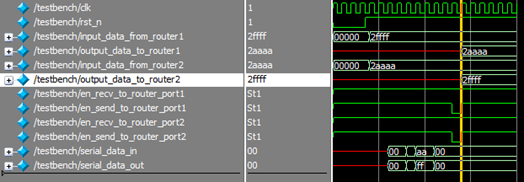
\includegraphics[scale=1]{./figs/phyTiming}
  \caption{\textbf{Timing Diagram of 2 Quasi-SERDES links cross connected}}
  \label{Quasi-SERDESLinkTiming}
\end{figure}

Quasi-SERDES link interface verifying the above performance parameters. 18 bit data injected in input port of one Quasi-SERDES link module appear at the output port of another Quasi-SERDES link module after 12 clock cycles. 

\section{Implementation Results}

This Quasi-SERDES link module compiled and synthesized for Altera and Xilinx devices. We have implemented the design on Altera Cyclone IV family device EP4CE22F17C6 \cite{DENanoManual} and uses 5632 logic elements and 56 GPIO pins. The large I/O requirement is when the module is implemented alone. The Quasi-SERDES link module is designed as an interface between two communicating nodes link two consecutive router in an NoC. When integrated with an NoC each of these modules added, adds 20 I/O's to the NoC design and approximately 5500 logical elements including registers for FIFO buffers. If NoC Quasi-SERDES link module system exceeds the available resources on the device these FIFO buffer can be resized to flit design.

\section{Limitations and improvements}
\begin{enumerate}
\item{Currently the Quasi-SERDES link module has not been very well optimized in regard with the hardware usage. Its a mechanical design which takes in n bits data as input and transmits 8 bits sending MSB first till the data is completely sent, similarly for receiving the module receives 8 bits and reconstructs the sent data from the transmitter.}
\item{The Quasi-SERDES link module sends read request and write request along with the transmitted data because of this there might be a scenario when data is misread or lost if these ready and acknowledge signals malfunction also This reduces the data rate as the transmitter can transmit at half the system clock. This a due to the reason that ready is high when data is ready to be sent and low for another cycle then again high for clock cycle when data ready to be sent and low for clock cycle which effective sends the complete data 8 bits at a time at half the system clock rate.} 
\end{enumerate}